%%%%%%%%%%%%%%%%%%%%%%%%%%%%%%%%%%%%%%%%%%%%%%%%%%%%%%%%%%%%%%%%%%%%%%%%%%%%%%%%%%%%%%%%%
% Section 11: Installing New Devices
%	This section provides a detailed walkthrough on how to install new devices
%	to be used in RapidSmith.
%%%%%%%%%%%%%%%%%%%%%%%%%%%%%%%%%%%%%%%%%%%%%%%%%%%%%%%%%%%%%%%%%%%%%%%%%%%%%%%%%%%%%%%%%
\newpage
\section{Installing New Device Files}
The device files included with the RapidSmith2 installation (listed in
\autoref{sec:supportedDevices}) have been well-tested, and are great starting
points for new users. If you are a new user, it is \emph{strongly encouraged}
that you learn RapidSmith's APIs and data structures by first implementing CAD tools on
these devices. However, RapidSmith2 also supports installing new device files
for parts not listed in \autoref{sec:supportedDevices}. This section contains
the following: (1) a description of the required intermediate files that need to be
generated from \texttt{Tincr} to support a new device, and (2) the necessary
steps to transform the intermediate files into compact device files that can be
loaded into RapidSmith2.

\subsection {XDLRC}
The \texttt{Device} data structures in RapidSmith are mainly created from XDLRC
files. XDLRC files contain a complete physical description of a Xilinx device
(including tiles, wires, sites, etc.). For older Xilinx parts (series 7 and
below), these files can be created in ISE with the \texttt{xdl} command. For
newer parts (UltraScale and above), XDLRC files can be created in Vivado using
the \texttt{Tincr} command \textit{tincr::write xdlrc}. Because XDLRC files can
grow to be hundreds of Gigabytes in size, RapidSmith compresses them into much smaller device files
(usually in the tens of Megabytes). \autoref{sec:appendixXDLRC} contains a more
detailed description of XDLRC syntax for those who are interested.

\subsection{FamilyInfo}
A \textit{familyInfo.xml} file contains useful information that is
not included in the XDLRC files for a given family of devices. Vivado currently 
supports 8 different family types: Artix7, Virtex7, Kintex7, Zynq, Kintex
UltraScale, Virtex UltraScale, Kintex UltraScale+, and Virtex UltraScale+. Only
one \textit{familyInfo.xml} file is required for each of these families (all 
devices within a family share the same family info). The remainder of this
section describes the important parts of a \textit{familyInfo.xml} file, and how
they are represented in RapidSmith2.

\begin{itemize}
  \item A list of \textbf{compatible types} for each site. Site A is said to be
  compatible with site B if the logical cells placed on site A can
  \textit{always} be placed on site B as well. For example, as shown in
  \autoref{fig:sliceCompatibility}, SLICEL sites are compatible with SLICEM
  sites. The cells placed on the SLICEL in the figure can be moved to the
  SLICEM and function indentically. SLICEM sites, however, are \textit{not}
  compatible with SLICEL sites. This is because SLICEM sites support LUT RAM
  cells, which cannot be placed on SLICEL sites.
  
  \begin{figure}[H]
    \centering
    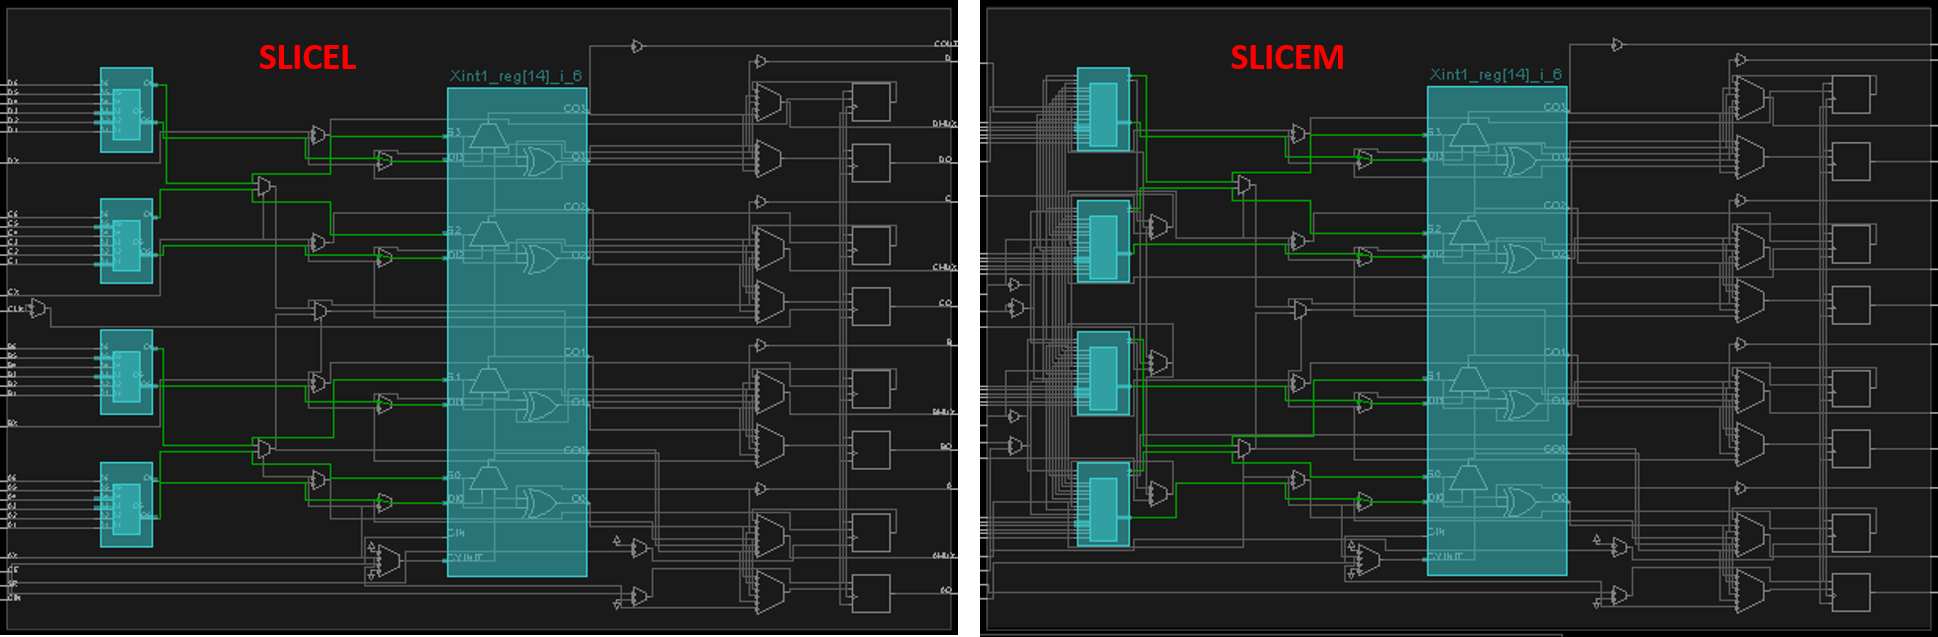
\includegraphics[width=1\columnwidth]{compatibleSites.png}
    \caption{The same group of cells placed on a SLICEL site (left) and a SLICEM
    site (right).}
    \label{fig:sliceCompatibility}
  \end{figure}
  
  \noindent Compatible sites are important
  to site-level placers in determining where a group of cells can be placed.
  \textbf{NOTE}: In some instances of compatibility, you have to first change
  the type of the compatible site before placing cells on it. For example, a
  RAMB36 site is compatible with a RAMBFIFO36 site. However, the site type of
  the RAMBFIFO36 site \textbf{must be changed to a RAMB36} before it is
  truly compatible.
  
  \item A list of \textbf{routethrough connections} for each LUT BEL (including
  the input bel-pin and output bel-pin of the routethrough). These routethrough
  connections are turned into \texttt{Connection} objects in RapidSmith2 that
  can be used for internal site routing. Sections \ref{sec:routing} and
  \ref{sec:additionalInfo} give more information about LUT routethroughs.
  
  \item A list of \textbf{alternate types} for each site. Each physical site on
  the device has an associated default type. Some sites, however, can be
  configured to be one of many types. An example for an UltraScale
  BITSLICE\_RX\_TX site is shown in \autoref{fig:alternateTypes}. As the figure
  shows, a BITSLICE\_RX\_TX site can also be configured to be of type
  BITSLICE\_COMPONENT\_RX\_TX, BITSLICE\_RXTX\_RX, or BITSLICE\_RXTX\_TX.
  RapidSmith2 parses the alternate site information from the XML and applies it
  to the corresponding \texttt{Site} data structure. This allows users to change
  site types based on what they need.
  
  \begin{figure}[H]
    \centering
    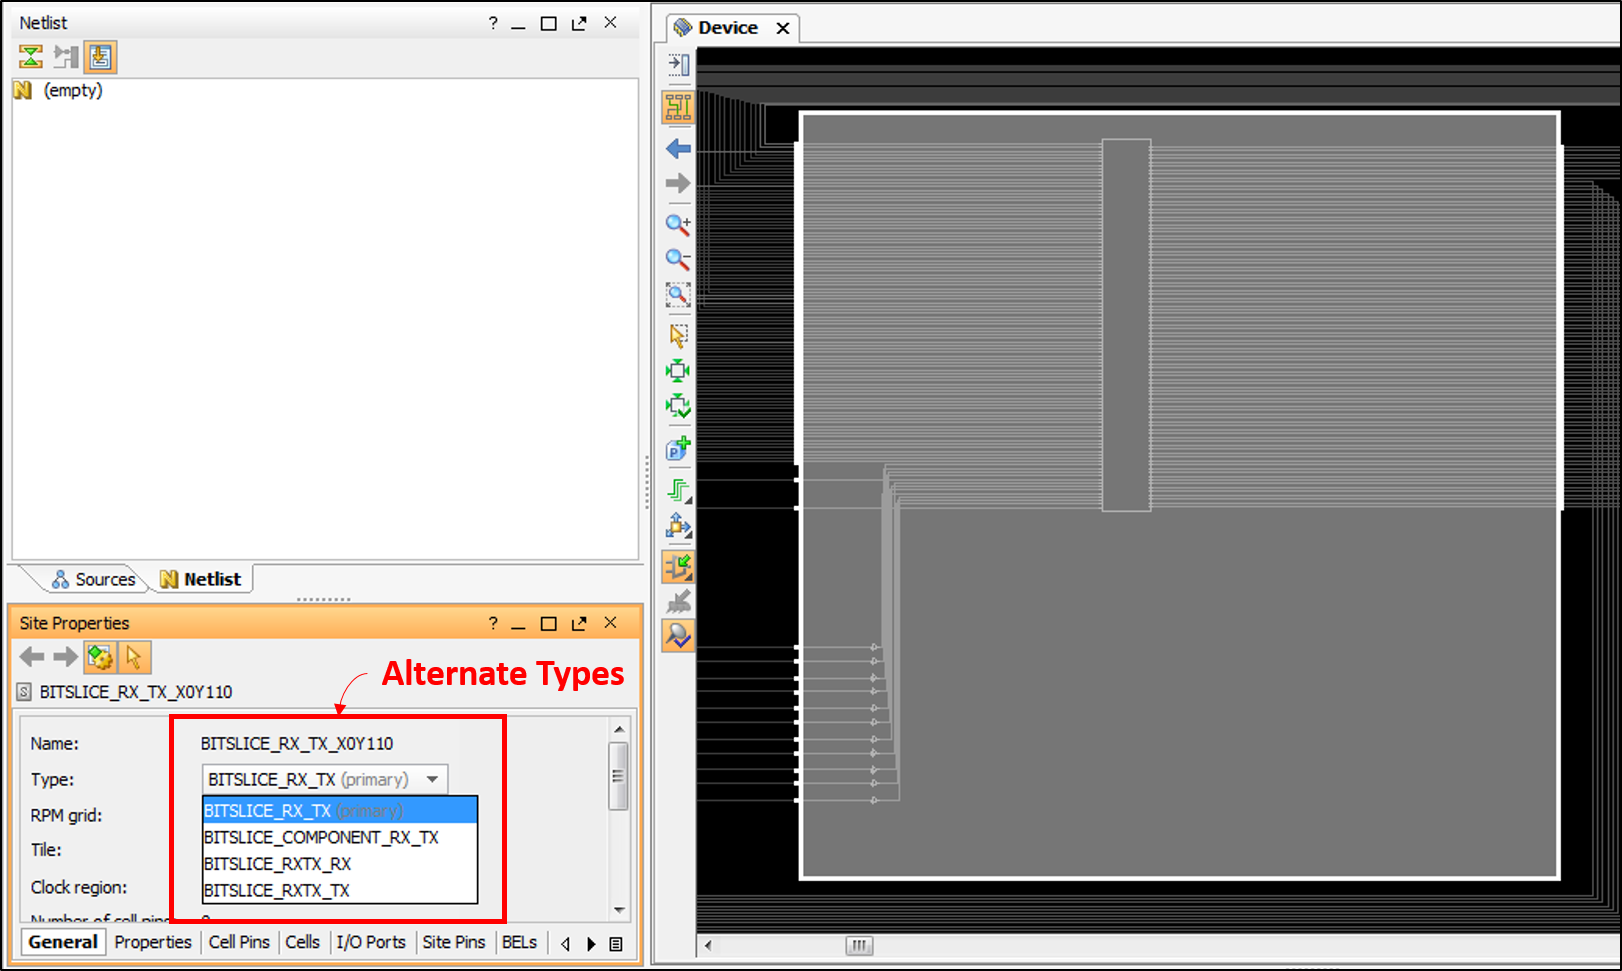
\includegraphics[width=.8\columnwidth]{alternateTypes.png}
    \caption{Vivado GUI showing alternate types for a BITSLICE\_RX\_TX site.}
    \label{fig:alternateTypes}
  \end{figure}
  
  \item A list of \textbf{site pip corrections}. In the XDLRC files that are
  parsed into RapidSmith, site pips (or routing muxes) are not distinguished
  from the functional BELs (such as LUTs and Flip Flops) of a site. The
  Family Info XML identifies the site pips of a site and marks them as either
  a ``mux'' or a ``polarity\_selector.'' RapidSmith2 transforms these routing
  muxes into individual pips as shown in \autoref{fig:sitePipDecomposition} so
  that they are no longer represented as BELs. After the decomposition, each pip
  is a routing resource of the site.
  
  \begin{figure}[H]
    \centering
    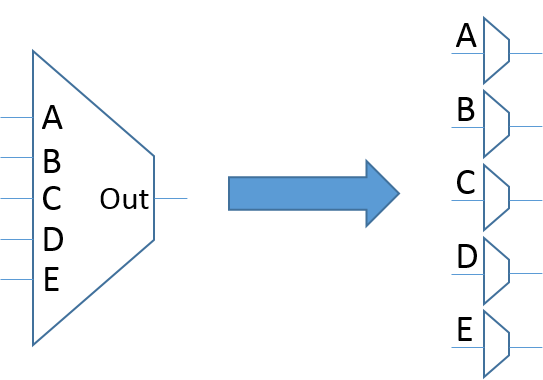
\includegraphics[width=.5\columnwidth]{sitePipDecomposition.png}
    \caption{RapidSmith2 site pip decomposition.}
    \label{fig:sitePipDecomposition}
  \end{figure}
  
  \item A list of \textbf{pin direction corrections}. For ISE-generated XDLRC
  files, all bel-pins are given a direction of either INPUT or OUTPUT. However,
  there are several bel-pins in Xilinx devices that are actually of direction
  INOUT (bidirectional). The Family Info file marks INOUT bel-pins so that
  their direction can be corrected in RapidSmith2.
  
\end{itemize}

\subsection{Creating New Device Files for Supported Families}
\autoref{sec:supportedDevices} gives a list of currently supported
families in RapidSmith2. If the device you want to install is \textbf{not}
within a supported family, see \autoref{sec:newFamilies} for how to add support for a
new family in RapidSmith. Otherwise, a new device file can be added in two easy
steps: 

\begin {enumerate}
\item Open Vivado in Tcl mode, and execute the \texttt{Tincr} command
\textit{::tincr::write\_xdlrc}. An example command usage is given below for the
Artix7 part \textit{xc7a100tcsg324-3}.

\begin{lstlisting}[numbers=none]
[ttown523@CB461-EE09968:�] vivado -mode tcl

****** Vivado v2014.2 (64-bit)
 **** SW Build 928826 on Thu Jun 5 17:55:10 MDT 2014
 **** IP Build 924643 on Fri May 30 09:20:16 MDT 2014
  ** Copyright 1986-2014 Xilinx, Inc. All Rights Reserved.

Vivado% ::tincr::write_xdlrc -part xc7a100tcsg324-3 -max_processes 4 -primitive_defs xc7a100tcsg324_full.xdlrc
\end{lstlisting}

\noindent The ``-max\_processes'' option is used to parallelize the operation so
that it will execute faster. If you have problems with the parallel generation
however (it can sometimes hang), then setting this option to ``1'' will
prevent the process from hanging. \textbf{NOTE}: This Tcl command can take a
very long time to run (more than 24 hours for very large devices). It is
suggested that you run it on a remote machine so that you can continue work on
your regular work machine. Also, be aware that these XDLRC files are massive. 100 GB
for the largest XDLRC files is not uncommon. Make sure you have enough space on
your hard drive before generating the XDLRC for a device.

\item Once the XDLRC creation is complete, run the device installer in
RapidSmith2 and pass the newly created XDLRC as an argument. An example command
line usage is shown below. The device installer can also be run in an IDE.

\begin{lstlisting}[numbers=none]
[ttown523@CB461-EE09968:�] java -ea -Xmx4096m edu.byu.ece.rapidSmith.util.Installer --generate file xc7a100tcsg324_full.xdlrc
\end{lstlisting} 

\noindent The device installer parses the verbose XDLRC file, and creates
compact RapidSmith device files (Megabytes instead of Gigabytes) that represent
a Xilinx device. Notice the two JVM command line arguments used in the command
above. The first option (``-ea'') enables assertions for the code. It is important
to include this flag so that device file errors can be caught during parsing.
If you are creating a new device file for a supported family however, there
should be no errors during the installation process. The second options
(``-Xmx4096m'') sets how much memory the JVM can use while running the
installer. Since XDLRC files are so large, the memory usage of the installer can
grow very quickly. In the command above, the JVM is set to use 4 GB of memory.
If the device installer fails with an out of memory exception, you will
need to increase the number of this parameter and re-run the installer (you may
need up to 32 GB of memory here).

\end{enumerate}

\noindent Once the device installer is done executing, the compact devices files
are stored in the corresponding family directory of the RapidSmith2 ``devices''
folder. For example, the device files generated from the example part
\textit{xc7a100tcsg324-3} are stored in the ``artix7'' sub-directory. The
listing below shows the two device files that are created after the device
installer is run (the device files are bolded). The file ending in ``\_db.dat''
contains the serialized \texttt{Device} data structures for RapidSmith. The file
ending in ``\_info.dat'' contains additional serialized data (such as reverse
wire connections) that can be optionally loaded with the device.

\begin{lstlisting}[numbers=none]
[ttown523@CB461-EE09968:artix7] ls
cellLibrary.xml familyInfo.xml |\textbf{xc7a100tcsg324\_db.dat}| |\textbf{xc7a100tcsg324\_info.dat}|
\end{lstlisting} 


\subsection{Supporting New Device Families} \label{sec:newFamilies}
 
1.) Look in the tincr/cache folder of your Tincr Installation. Then try to find
the family folder for you device (i.e. Artix7). If you look inside the family
folder and there is no ``primitive defs'' folder (or the family folder does not
exist), then you will need to generate the primitive defs before creating the
XDLRC file. To do this, you will need to use the VSRT GUI. The process to
create a new set of primitive defs is given in the VSRTUserGuide.pdf of the RS2
repository. 

2.) Once the primitive defs are created, put them in the tincr cache folder as
described in step (1). 

% TODO: put full command here!
3.) Run the Tincr command ::tincr::write\_xdlrc - 
where ``myPart'' is replaced with the part of your choice

4.) Look in the RapidSmith2 directory devices/family. If there is a
familyInfo.xml file already there, then you don't have to worry about creating a
new one yourself. Skip to step ?

5.) Generate a new Family Info. If you are generating a new familyInfo.xml, then
that means that most likely you also generated the primitive defs using VSRT. In
the VSRT folder you used, there is a file called ``addedBels.txt''.
To generate a new family info file, run the Vivado command
::tincr::create\_xml\_family\_info ``familyInfo.xml'' family addedBels.txt. 
This will generate most of the information you need for the family info file.
However, there are some compatible sites that are NOT included with this file. 
For ultrascale, we needed to manually add these two compatible types manually:
!!put pictures here with highlighted text!!
For your device, you will have to determine what compatible types are missing
(SLICEL->SLICEM will always be one, and there should be some IOB sites that are
compatible, but the rest is up to you to determine). It is best practice to go
through each site in the family info file, and make sure there are no
corrections that need to be made before creating a new device file in
RApidSmith. Once the family info is created, store it in
rapidSmithPath/devices/family/familyInfo.xml. 

6.) To generate a new device file in RS2, you need to execute the java class
with the following options  ``ece.byu.edu.rapidSmith.util.Installer --generate
file pathToXDLRCFile''. This process requires A LOT of memory. Make sure that
you enable assertions (-ea) and set the max memory usage of the Installer
(-Xmx8000m) to a number big enough. Having at least 16 GB of RAM is recommended
for this process. If the installer fails because you ran out of memory, keep
increasing the memory until it does not fail. 

\begin{enumerate}
  \item 
\end{enumerate}

